% -------------------------------------------------------------------
% A simple LaTeX book template
% -------------------------------------------------------------------
\documentclass{lifmanual}
\usepackage{import}

% Generate an index
\makeindex%[intoc]

% ---------------------------------------
% The gitbook-pandoc script will generate a file
% called pandoc.inc.tex, which contains many declarations
% required to compile the book.
% ---------------------------------------
% Here we use a frozen version of pandoc.inc.tex, as we made a few
% modifications to the Pandoc-generated file
\input{pandoc.inc.freeze.tex}

% ---------------------------------------
% Title and author
% ---------------------------------------
\title{Event Stream Processing with BeepBeep}
\author{Sylvain Hallé}
\hypersetup{
  pdftitle = {Event Stream Processing with BeepBeep},
  pdfauthor = {Sylvain Hallé}
}
\usepackage{multicol}

% Allow hyphenation in tt font
% found from https://tex.stackexchange.com/a/44362/165194
\DeclareFontFamily{\encodingdefault}{\ttdefault}{\hyphenchar\font=`\-}
%\hyphenation{Pro-ces-sor}

% Define the "pencil" character to place below code snippets
\usepackage{newunicodechar}
\DeclareUnicodeCharacter{2693}{\ding{46}}

% Command for showing palette icon in glossary
\newcommand{\bbpalette}[1]{\hspace{-1em}\includegraphics[height=2.5mm]{chapters/dictionary/Palette-#1}\phantom{W}}

\begin{document}
\frontmatter
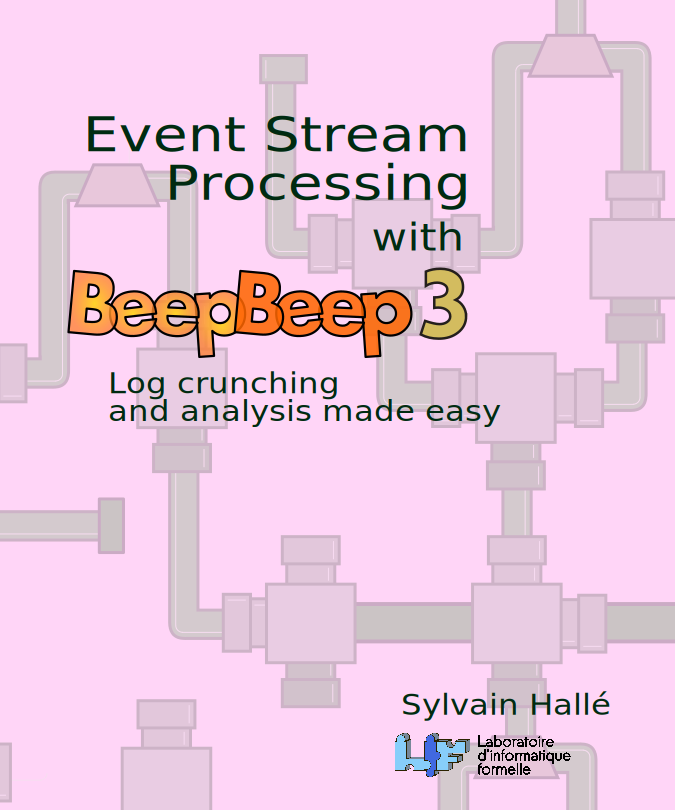
\includepdf[width=7.5in,height=9in]{Cover.pdf}
\newpage

\cleardoublepage
\includepdf[width=7.5in,height=9in]{Cover-inside.pdf}
\newpage

%% 2nd cover
\thispagestyle{empty}
\pagestyle{empty}
\rule{0in}{6in}
\noindent
\includegraphics[width=1in]{by-nc-nd}\\
{\sf\small
\noindent
This work is licensed under the Creative Commons Attribution-NonCommercial-NoDerivatives 4.0 International License. To view a copy of this license, visit \url{http://creativecommons.org/licenses/by-nc-nd/4.0/}.\\

\noindent
\rule{0in}{8pt}
\noindent
Book version: L1.1---August 10, 2018}


\tableofcontents
\newpage

\mainmatter
\thispagestyle{normal}
\pagestyle{normal}

\subimport*{chapters/}{body}

\appendix
% Change "chapter" for "appendix" in footer for these chapters
\renewcommand{\chaptername}{Appendix}
\setcounter{tocdepth}{0} % No sections in TOC
\subimport*{chapters/}{drawing/README}
\subimport*{chapters/}{dictionary/README}

%% Change footer for index
\pagestyle{index}
\printindex

%% Back of the book
\cleardoublepage
\thispagestyle{empty}
\phantom{W}
\newpage
\includepdf[width=7.5in,height=9in]{Cover-outside.pdf}

\end{document}
%% :wrap=soft: